\section{CROSS INDUSTRY STANDARD PROCESS FOR DATA MINING (CRISP-DM)}

Según \parencite{wirth2000crisp} la metodología \textit{CRISP-DM} proveé una visión general del ciclo de vida de un proyecto basado en \textit{Minería de Datos}. Este ciclo de vida se descompone en seis fases: \textit{Entendimiento del Negocio}, \textit{Entendimiento de los Datos}, \textit{Preparación de los Datos}, \textit{Modelado}, \textit{Evaluación} y \textit{Despliegue}. Estas fases siguen un proceso secuencial no estricto y se puede adaptar a las necesidades del proyecto, sin embargo, existe una secuencia frecuente basada en las dependencias de cada fase.

En el contexto del proyecto actual, las metodologías basadas en Minería de Datos deben ser tomadas en cuenta debido a que los Sistemas de Recomendación forman parte del ámbito de dicha disciplina y, \textit{CRISP-DM} ha sido diseñado para estructurar proyectos de Minería de Datos sin establecer un objetivo en específico (clasificación, clustering, regresión, recomendación).

\begin{figure}[h!]
    \centering
    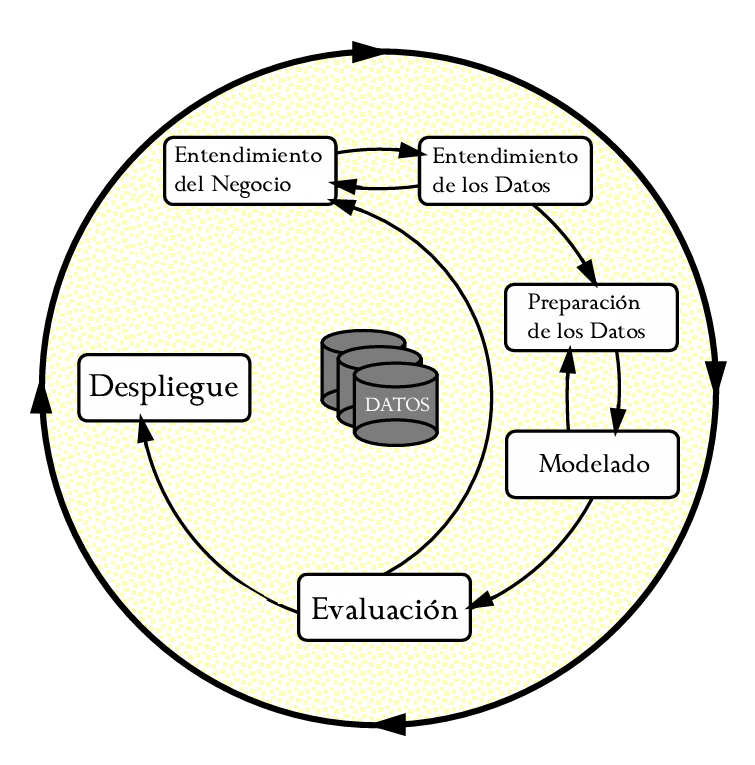
\includegraphics[width=0.65\linewidth]{CRISPDM.png}
    \caption{Fases de la Metodología CRISP-DM \parencite{wirth2000crisp}.}
    \label{fig:FasesCRISPDM}
\end{figure}

En la figura \Cref{fig:FasesCRISPDM} se puede visualizar que las fases de \textit{CRISP-DM} son cíclicas debido a la naturaleza de la \textit{Minería de Datos}, ya que estos se retroalimentan de sus propios resultados, ya sean errores o aciertos.

Cada una de las fases que componen a la metodología \textit{CRISP-DM} cumplen con un propósito específico, a continuación se describe la función de cada una de las fases basándose en \parencite{schroer2021systematic} y \parencite{wirth2000crisp}.

\textbf{FASE 1: ENTENDIMIENTO DEL NEGOCIO}

La fase inicial denominada como \textit{Entendimiento del Negocio} se enfoca en entender los objetivos y requerimientos del proyecto, convirtiéndo este conocimiento en la definición de un problema a resolver mediante \textit{Minería de Datos} y en un plan de proyecto preliminar diseñado para cumplir dichos objetivos.

La situación del negocio debe ser evaluada para obtener una visión general de los recursos necesarios. Uno de los puntos más importantes de esta fase es la determinación del \textbf{Objetivo de la Minería de Datos}. El primer paso es definir el tipo de Minería de Datos que se desarrollará (en este caso, Recomendación) y el criterio de éxito. 

\textbf{FASE 2: ENTENDIMIENTO DE LOS DATOS}

La fase de \textit{Entendimiento de los Datos} empieza con una colección de datos inicial y es seguida de actividades que fomenten el entendimiento de los datos para identificar problemas de calidad, descubrir perspectivas iniciales o detectar subcolecciones para identificar información escondida.

\textbf{FASE 3: PREPARACIÓN DE LOS DATOS}

La fase de \textit{Preparación de los Datos} se enfoca en construir el \textit{Dataset} final en base a la primera recolección de datos. Estas tareas de preparación se deben ejecutar múltiples veces. Estas actividades incluyen tareas de selección de tablas, limpieza de datos, construcción de nuevos atributos y transformación de datos para herramientas de modelado.

Además, se debe realizar un proceso de selección de datos definiendo criteros de inclusión y exclusión. Los datos de mala calidad deben ser procesados mediante una tarea de limpieza de datos.

\textbf{FASE 4: MODELADO}

Esta fase consiste en seleccionar una técnica de minería de datos dependiendo el problema del negocio y los datos disponibles. En general, se pueden usar todas las técnicas siempre y cuando se justifiquen a través de criterios de evaluación, o de lo contrario, es recomendable evaluar el rendimiento de diferentes técnicas y determinar a los que lograron un mejor rendimiento.

\textbf{FASE 5: EVALUACIÓN}

En este momento del desarrollo ya se tiene uno o más modelos que aparentan buena calidad desde un punto de vista analítico. Sin embargo, antes de proceder al despliegue es importante evaluar profundamente al sistema, principalmente identificando si existe algún objetivo del negocio que no ha sido cumplido satisfactoriamente.
Además de evaluar al sistema a profundidad, también se debe evaluar el proceso de desarrollo llevado a cabo.

\textbf{FASE 6: DESPLIEGUE}

La creación del modelo generalmente no representa el final del proyecto, por el contrario, la experiencia obtenida en el uso de diferentes modelos de Minería de Datos debe ser organizada y reportada de forma detallada para elaborar manuales de usuario. Sin embargo, esta fase puede ser tan simple como generar un reporte de usuario o tan complejo como aplicar diferentes procesos de Minería de Datos. 

En muchos casos, el usuario final será el encargado del despliegue y no el analísta de datos. 